\documentclass[12pt]{article}
\usepackage[pdftex]{graphicx}
\usepackage[finnish]{babel}
\usepackage[utf8]{inputenc}
\usepackage{amsfonts}
\usepackage{amsmath}
\usepackage{amssymb}
\usepackage{color}

\begin{document}

\Huge{\bf{Ohjelmoinnin harjoitustyö}}

\normalsize

\section{Aiheen kuvaus}

\paragraph{Kahden pelaajan shakki}

\paragraph{} Toteutetaan ohjelma, joka mallintaa shakin pelilautaa, nappuloita ja sääntöjä. Pelaaja voi siirtää nappuloita shakin sääntöjen mukaisesti. Ohjelma ei sisällä tietokonevastustajaa.

\begin{itemize}

\item Ohjelma sallii vain sääntöjen mukaiset siirrot

\item Ohjelma sallii paitsi kaikki tavalliset siirrot myös
\begin{itemize}
\item kaappauksen,
\item tornituksen,
\item sivustalyönnin ja
\item sotilaan korottuminen
\end{itemize}

\item Ohjelma tunnistaa, milloin kuningas on shakattu

\item Käyttöliittymä mahdollistaa
\begin{itemize}
\item siirtojen tekemisen,
\item uuden pelin aloittamisen,
\item siirtojen perumisen (undo),
\item vapaa pelitilanteeseen siirtyminen (FEN) ja
\item pelin lopettamisen
\end{itemize}

\item Käyttöliittymä on tekstipohjainen ja pelitilanteesta esitetään vähiintään
\begin{itemize}
\item pelilaudan tilanne,
\item siirtovuoro,
\item siirtojen lukumäärä,
\item materiaalin määrä molemmilla pelaajilla ja
\item viidenkymmenen siirron säännön voimassaolo
\end{itemize}

\item Ohjelma on yhteensopiva seuraavien käytäntöjen kanssa:
\begin{itemize}
\item Standard Algebraic Notation, jota käytetään siirtojen tekemiseen
\item Forsyth-Edwards Notation, jonka ohjelma osaa tulostaa ja parsia
\end{itemize}

\end{itemize}

\section{Ohjelman rakenne}

\paragraph{} Ohjelma on jaettavissa kahteen osaan, jotka ovat käyttöliittymä ja pelilogiikka. Käyttöliittymä on pieni ja yksinkertainen komentorivipohjainen ratkaisu, joka on toteutettu yhdessä ainoassa luokassa.

\paragraph{} Pelilogiikka sen sijaan on jaettu useisiin luokkiin ja ne voidaan toiminan mukaan jakaa kahteen pääryhmään: pää- ja apuluokkiin. Pääluokat on seuraavan sivun kaaviokuvassa merkitty keskelle (Chess, Board ja Piece) ja tavallisesti ohjelman suoritus virtaa kaaviossa ylhäältä alas ja takaisin ylös. Esimerkiksi yksi tavallisimmista ohjelman toiminnoista on siirron tekeminen pelilaudalla. Tällöinkäyttöliittymä antaa käyttäjän syötteen Chess-luokalle, joka Move-luokan avulla parsii syötteen. Tämän jälkeen suoritus siirretään Board-luokalle ja (mahdollisten apuluokkien jälkeen) Piece-luokalle.

\paragraph{} Apuluokkia (Castle, Coord, Move ja Rebound) käytetään tarpeen mukaan. Esimerkiksi Castle-luokkaa tarvitaan erityisesti silloin, kun pelaajan tekemä siirto on tornitus.

\paragraph{} Piece on geneerinen pelinappulan yliluokka, jolla on joukko aliluokkia - tarkalleen ottaen luokat BlackBishop, BlackKing, BlackKnight, BlackPawn, BlackQueen, BlackRook, WhiteBishop, WhiteKing, WhiteKnight, WhitePawn, WhiteQueen ja WhiteRook. Aliluokat vastaavat shakkipelin erillaisia nappuloita omine sääntöineen.

\paragraph{} Edellämainittujen lisäksi ohjelma hyödyntää kahta enum-rakennetta sekä virheenkäsittelyssä auttavaa MoveException-luokkaa (ei kaaviossa).

\newpage

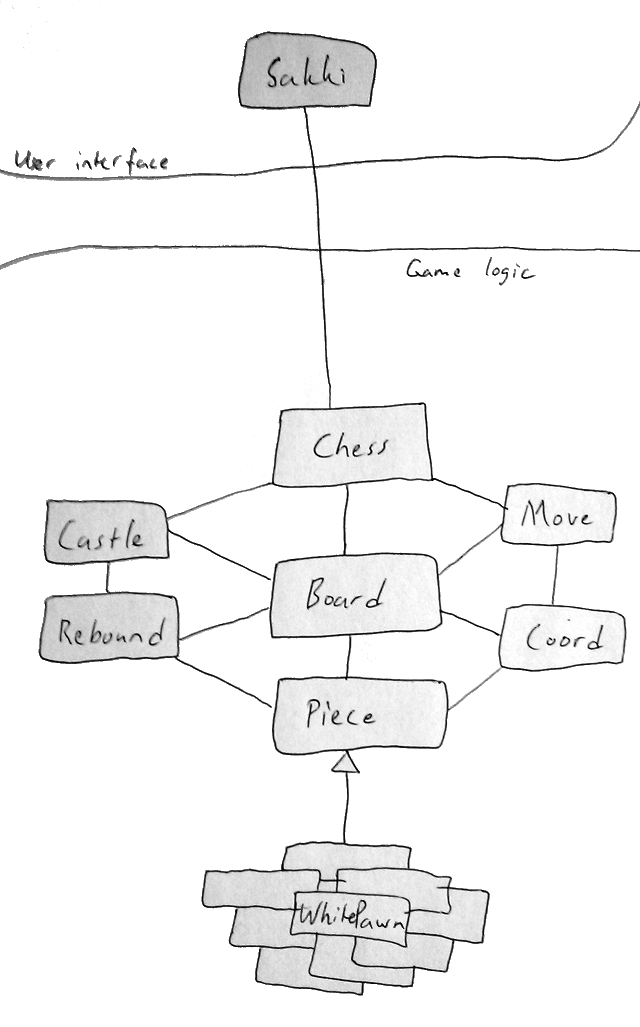
\includegraphics[height=210mm]{luokkakaavio.png}

\end{document}
